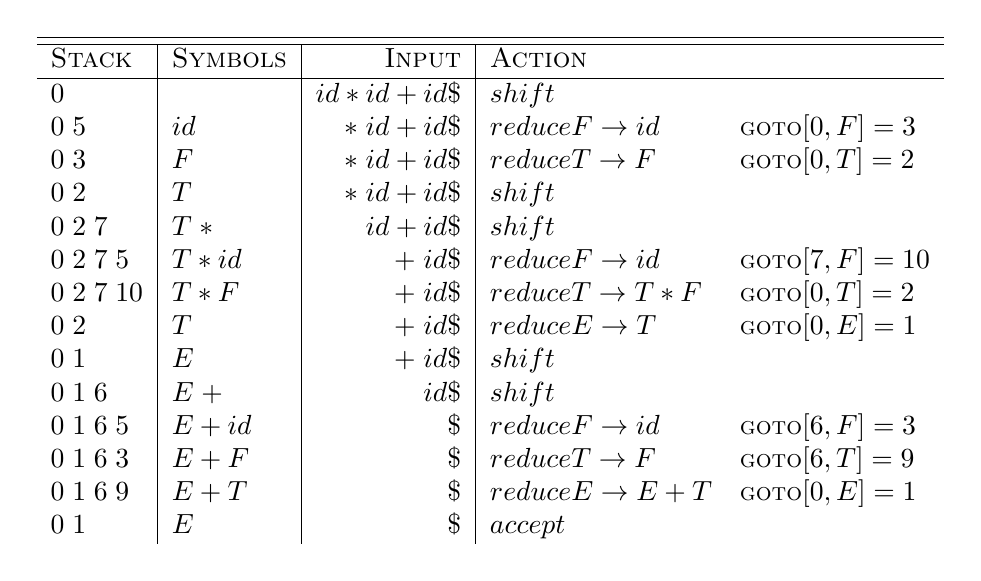
\begin{tikzpicture}
\node (table) {$\begin{array}{l|l|r|ll}
\hline\hline
\textsc{Stack} & \textsc{Symbols} & \textsc{Input} & \textsc{Action} \\
\hline
 0        &        & \text{id} * \text{id} + \text{id} \$ & \text{shift}                 \\
 0\; 5      & \text{id}     & *\;\text{id} + \text{id} \$    & \text{reduce } F \to \text{id} &  {\small \textsc{goto}[0,F] = 3 } \\
 0\; 3      & F      & *\;\text{id} + \text{id} \$    & \text{reduce } T \to F&  {\small \textsc{goto}[0,T] = 2   } \\
 0\; 2      & T      & *\;\text{id} + \text{id} \$    & \text{shift}                 \\
 0\; 2\; 7    & T\;*    & \text{id} + \text{id} \$      & \text{shift}                 \\
 0\; 2\; 7\; 5  & T * \text{id} & +\;\text{id} \$         & \text{reduce } F \to \text{id}&  {\small \textsc{goto}[7,F] = 10  } \\
 0\; 2\; 7\; 10 & T * F  & +\;\text{id} \$         & \text{reduce } T \to T * F&  {\small \textsc{goto}[0,T] = 2} \\
 0\; 2      & T      & +\;\text{id} \$         & \text{reduce } E \to T &  {\small \textsc{goto}[0,E] = 1  } \\
 0\; 1      & E      & +\;\text{id} \$         & \text{shift}                 \\
0\; 1\; 6    & E\;+    & \text{id} \$           & \text{shift}                 \\
0\; 1\; 6\; 5  & E + \text{id} & \$              & \text{reduce } F \to \text{id}&  {\small \textsc{goto}[6,F] = 3   } \\
0\; 1\; 6\; 3  & E + F  & \$              & \text{reduce } T \to F &  {\small \textsc{goto}[6,T] = 9  } \\
0\; 1\; 6\; 9  & E + T  & \$              & \text{reduce } E \to E + T&  {\small \textsc{goto}[0,E] = 1} \\
0\; 1      & E      & \$              & \text{accept}
\end{array}$};
\end{tikzpicture}
